\chapter{Udara, Campuran Gas}\label{ch:g4:air-a-mixture-of-gases}

Pada hari berangin, layang-layang menarik-narik benangnya, dan di danau
sebuah layar mengembang dan mendorong perahu. Ada sesuatu yang mendorong
keduanya, padahal tidak ada yang terlihat. Sesuatu itu adalah \omterm{def:g4:air-a-mixture-of-gases:air}{udara}.
Kita tidak dapat melihatnya, tetapi \omterm{def:g4:air-a-mixture-of-gases:air}{udara} ada di sekeliling kita, mengisi
setiap botol kosong dan setiap ruangan, dan kita menghirupnya setiap
kali bernapas. Terbuat dari apakah \omterm{def:g4:air-a-mixture-of-gases:air}{udara}?

\begin{recall}
\omterm{def:g2:mixing-and-dissolving:mix}{Mencampur} berarti menyatukan benda-benda yang berbeda; yang kita peroleh
adalah campuran benda-benda itu, dan tidak ada yang hilang ketika kita
\omterm{def:g2:mixing-and-dissolving:mix}{mencampurnya} (\cref{ch:g2:mixing-and-dissolving}).
\end{recall}

\begin{omfigure}
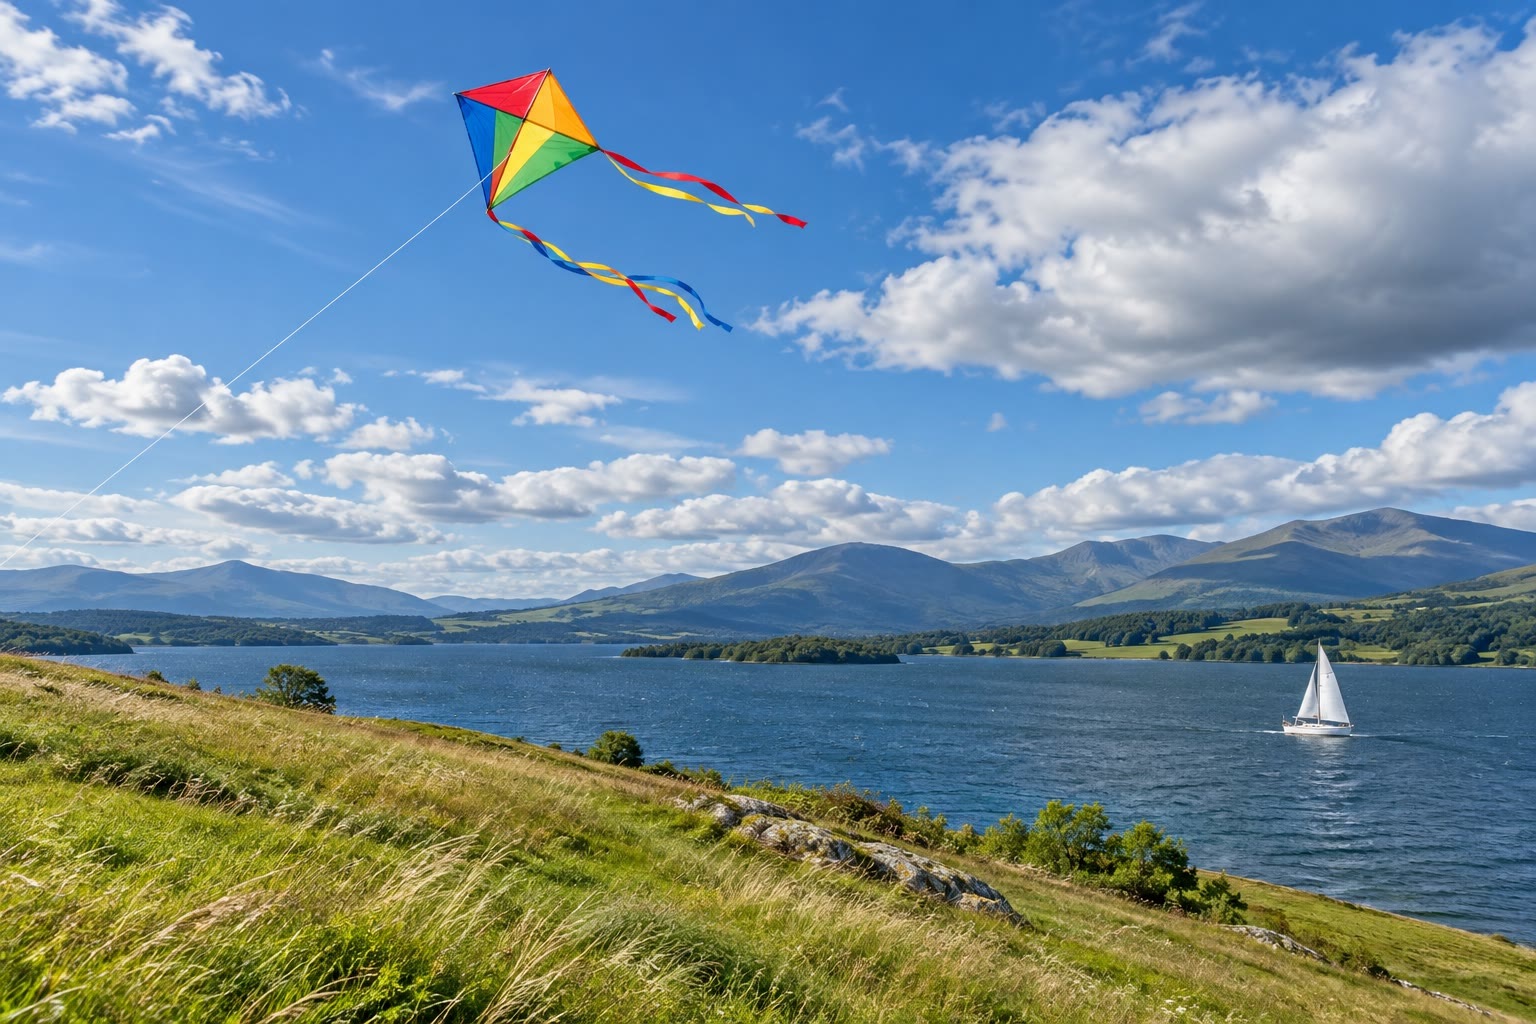
\includegraphics[width=0.6\linewidth]{images/book1/ai/g4-kite-day.jpg}

{\small Layang-layang dan layar: \omterm{def:g4:air-a-mixture-of-gases:air}{udara} tidak terlihat, tetapi \omterm{def:g4:air-a-mixture-of-gases:air}{udara} mendorong.}
\end{omfigure}

\section{Udara ada di sekeliling kita}

\begin{example}[Gelas terbalik]\label{ex:g4:air-a-mixture-of-gases:glass}
Selembar tisu kering dijejalkan ke dasar sebuah gelas kosong. Gelas itu
dibalik lalu ditekan lurus ke bawah ke dalam baskom berisi air. Ketika
diangkat lagi, tisunya tetap kering. Gelas itu tidak kosong: gelas itu
penuh \omterm{def:g4:air-a-mixture-of-gases:air}{udara}, dan udaralah yang menahan air agar tidak masuk.
\end{example}

\begin{omfigure}
\begin{tikzpicture}[font=\small, scale=1.3]
  \pic[transform shape] at (0,0) {trough};
  % the upturned glass, rim at y = 0.35, base at y = 2.35
  \fill[white] (-0.8,0.5) rectangle (0.8,0.95);
  \pic[transform shape, rotate=180] at (0,2.35) {beaker={0}{white}};
  % the tissue at the top, inside
  \fill[white, draw=black!45, rounded corners=1.5pt] (-0.4,2.33) -- (-0.3,2.05)
    -- (-0.1,2.12) -- (0.05,1.98) -- (0.25,2.1) -- (0.42,2.02) -- (0.45,2.33) -- cycle;
  \draw[<-, omProp, thick] (0.45,2.12) -- (2.4,2.5) node[right, text=black]
    {tisu kering};
  \draw[<-, omProp, thick] (0.3,1.2) -- (2.4,1.4) node[right, text=black]
    {udara: menahan air agar tidak masuk};
  \draw[<-, omProp, thick] (1.4,0.7) -- (2.4,0.55) node[right, text=black]
    {air};
\end{tikzpicture}

{\small Gelas ditekan terbalik ke dalam air. \omterm{def:g4:air-a-mixture-of-gases:air}{Udara} yang terperangkap di
dalamnya menahan air agar tidak masuk, dan tisunya tetap kering.}
\end{omfigure}


\begin{remark}[Udara adalah gas]\label{rem:g4:air-a-mixture-of-gases:gas}
\omterm{def:g4:air-a-mixture-of-gases:air}{Udara} adalah gas: \omterm{def:g4:air-a-mixture-of-gases:air}{udara} tidak punya bentuk sendiri dan menyebar mengisi
wadah apa pun. Meskipun begitu, \omterm{def:g4:air-a-mixture-of-gases:air}{udara} tetap materi, dan balon yang penuh
\omterm{def:g4:air-a-mixture-of-gases:air}{udara} sedikit lebih berat daripada balon yang sama dalam keadaan kosong.
Apa itu gas, dan mengapa gas berperilaku begini, diceritakan di buku
fisika.
\end{remark}

\section{Udara adalah campuran}

\begin{definition}[Udara]\label{def:g4:air-a-mixture-of-gases:air}
Yang disebut \emph{udara}\index{udara} adalah campuran gas yang
menyelimuti Bumi. Udara bukan satu gas saja: beberapa gas bercampur di
dalamnya, dan gas-gas itu dapat dipisahkan satu dari yang lain.
\end{definition}

\begin{proposition}[Penyusun udara]\label{prop:g4:air-a-mixture-of-gases:composition}
% ledger: air:N2, air:O2, air:Ar, air:trace, air:CO2, air:H2O
Tanpa menghitung uap airnya, \omterm{def:g4:air-a-mixture-of-gases:air}{udara} terdiri atas:
\begin{itemize}
  \item \textbf{nitrogen}, sekitar empat perlima \omterm{def:g4:air-a-mixture-of-gases:air}{udara};
  \item \textbf{oksigen}, sekitar seperlima \omterm{def:g4:air-a-mixture-of-gases:air}{udara};
  \item sedikit \textbf{argon}, sekitar 1 bagian per 100;
  \item sedikit sekali \textbf{karbon dioksida}, sekitar 4 bagian per
        10\,000, dan sejumlah kecil gas lain.
\end{itemize}
\omterm{def:g4:air-a-mixture-of-gases:air}{Udara} juga mengandung \textbf{uap air} yang tidak terlihat: sangat
sedikit pada hari yang kering dan dingin, sampai sekitar 4 bagian per
100 pada hari yang panas dan lembap.
\end{proposition}

\begin{example}[Seratus botol udara]\label{ex:g4:air-a-mixture-of-gases:hundred}
% ledger: air:N2, air:O2, air:Ar
Bayangkan 100 botol \omterm{def:g4:air-a-mixture-of-gases:air}{udara} kering, dan gas-gas \omterm{def:g4:air-a-mixture-of-gases:air}{udara} itu dipilah ke dalam
botol-botol terpisah. Sekitar 78 botol akan berisi nitrogen, 21 botol
oksigen, dan botol terakhir argon, ditambah karbon dioksida dan gas lain
yang hanya setara beberapa tetes.
\end{example}

\begin{omfigure}
\begin{tikzpicture}[font=\small, x=0.42cm, y=0.42cm]
  \foreach \k in {0,...,99} {
    \pgfmathtruncatemacro\col{mod(\k,10)}
    \pgfmathtruncatemacro\row{9-int(\k/10)}
    \ifnum\k<78 \def\c{omDef!45}\else\ifnum\k<99 \def\c{red!45}\else\def\c{cyan!60}\fi\fi
    \fill[\c, draw=white, line width=0.8pt] (\col,\row) rectangle ++(1,1);
  }
  \fill[omDef!45] (12,8) rectangle ++(1,1);
  \node[anchor=west] at (13.3,8.5) {nitrogen: 78 kotak};
  \fill[red!45] (12,6) rectangle ++(1,1);
  \node[anchor=west] at (13.3,6.5) {oksigen: 21 kotak};
  \fill[cyan!60] (12,4) rectangle ++(1,1);
  \node[anchor=west, align=left] at (13.3,4.5) {argon, karbon dioksida\\ dan sisanya: 1 kotak};
\end{tikzpicture}

{\small Seratus kotak \omterm{def:g4:air-a-mixture-of-gases:air}{udara} kering. Kotak di kanan bawah berisi argon,
dan karbon dioksida yang terlalu sedikit untuk digambar tersendiri.}
\end{omfigure}

\begin{remark}[Nama-nama gas]\label{rem:g4:air-a-mixture-of-gases:names}
Nitrogen, oksigen, argon, dan karbon dioksida adalah nama-nama gas.
Semuanya tidak berwarna dan tidak berbau. Sebuah bab berikutnya
menunjukkan dari apa masing-masing gas itu tersusun, sampai ke
kepingan-kepingan sangat kecil yang menyusun semua materi.
\end{remark}

\section{Yang kita hirup dan kita embuskan}

\begin{proposition}[Udara embusan napas]\label{prop:g4:air-a-mixture-of-gases:breath}
% ledger: breath:O2, breath:CO2, breath:N2, air:O2, air:CO2
\omterm{def:g4:air-a-mixture-of-gases:air}{Udara} yang kita embuskan bukan \omterm{def:g4:air-a-mixture-of-gases:air}{udara} yang kita hirup. Tubuh kita
mengambil sebagian oksigennya dan mengeluarkan karbon dioksida dan uap
air:
\begin{itemize}
  \item sekitar 21 bagian per 100 \omterm{def:g4:air-a-mixture-of-gases:air}{udara} yang dihirup adalah oksigen,
        tetapi hanya sekitar 16 bagian per 100 \omterm{def:g4:air-a-mixture-of-gases:air}{udara} yang diembuskan;
  \item karbon dioksida naik dari sekitar 4 bagian per 10\,000 menjadi
        sekitar 4 bagian per 100: kira-kira seratus kali lebih banyak;
  \item nitrogen diembuskan sama persis seperti saat dihirup.
\end{itemize}
\end{proposition}

\begin{omfigure}
\begin{tikzpicture}
\begin{axis}[ybar, width=0.8\linewidth, height=5.2cm, bar width=12pt,
    ymin=0, ymax=90, ylabel={bagian per 100},
    symbolic x coords={nitrogen, oxygen, carbon dioxide}, xtick=data,
    xticklabels={nitrogen, oksigen, karbon dioksida},
    tick label style={font=\small}, label style={font=\small},
    xticklabel style={text height=1.6ex, text depth=0.4ex},
    legend style={font=\small, at={(0.98,0.95)}, anchor=north east},
    nodes near coords, nodes near coords style={font=\footnotesize},
    enlarge x limits=0.25, axis lines*=left, ymajorgrids,
    grid style={gray!20}]
% ledger: air:N2, air:O2, air:CO2, breath:N2, breath:O2, breath:CO2 (rounded)
\addplot[fill=omDef!45, draw=omDef] coordinates
  {(nitrogen,78) (oxygen,21) (carbon dioxide,0)};
\addplot[fill=omProp!55, draw=omProp] coordinates
  {(nitrogen,78) (oxygen,16) (carbon dioxide,4)};
\legend{dihirup, diembuskan}
\end{axis}
\end{tikzpicture}

{\small \omterm{def:g4:air-a-mixture-of-gases:air}{Udara} yang dihirup dan yang diembuskan, dalam bagian per 100
(tanpa uap air, angka dibulatkan). Karbon dioksida dalam \omterm{def:g4:air-a-mixture-of-gases:air}{udara} yang
dihirup, 4 bagian per 10\,000, terlalu sedikit untuk ditampilkan
sebagai batang.}
\end{omfigure}

\begin{example}[Ruangan yang penuh orang]\label{ex:g4:air-a-mixture-of-gases:room}
Di sebuah ruang kelas kecil yang jendelanya tertutup, tiga puluh orang
mengembuskan karbon dioksida sepanjang pagi. Sedikit demi sedikit \omterm{def:g4:air-a-mixture-of-gases:air}{udara}
di ruangan itu mengandung lebih sedikit oksigen dan lebih banyak karbon
dioksida, dan orang-orang merasa lelah. Membuka jendela memasukkan
kembali \omterm{def:g4:air-a-mixture-of-gases:air}{udara} segar.
\end{example}

\begin{omfigure}
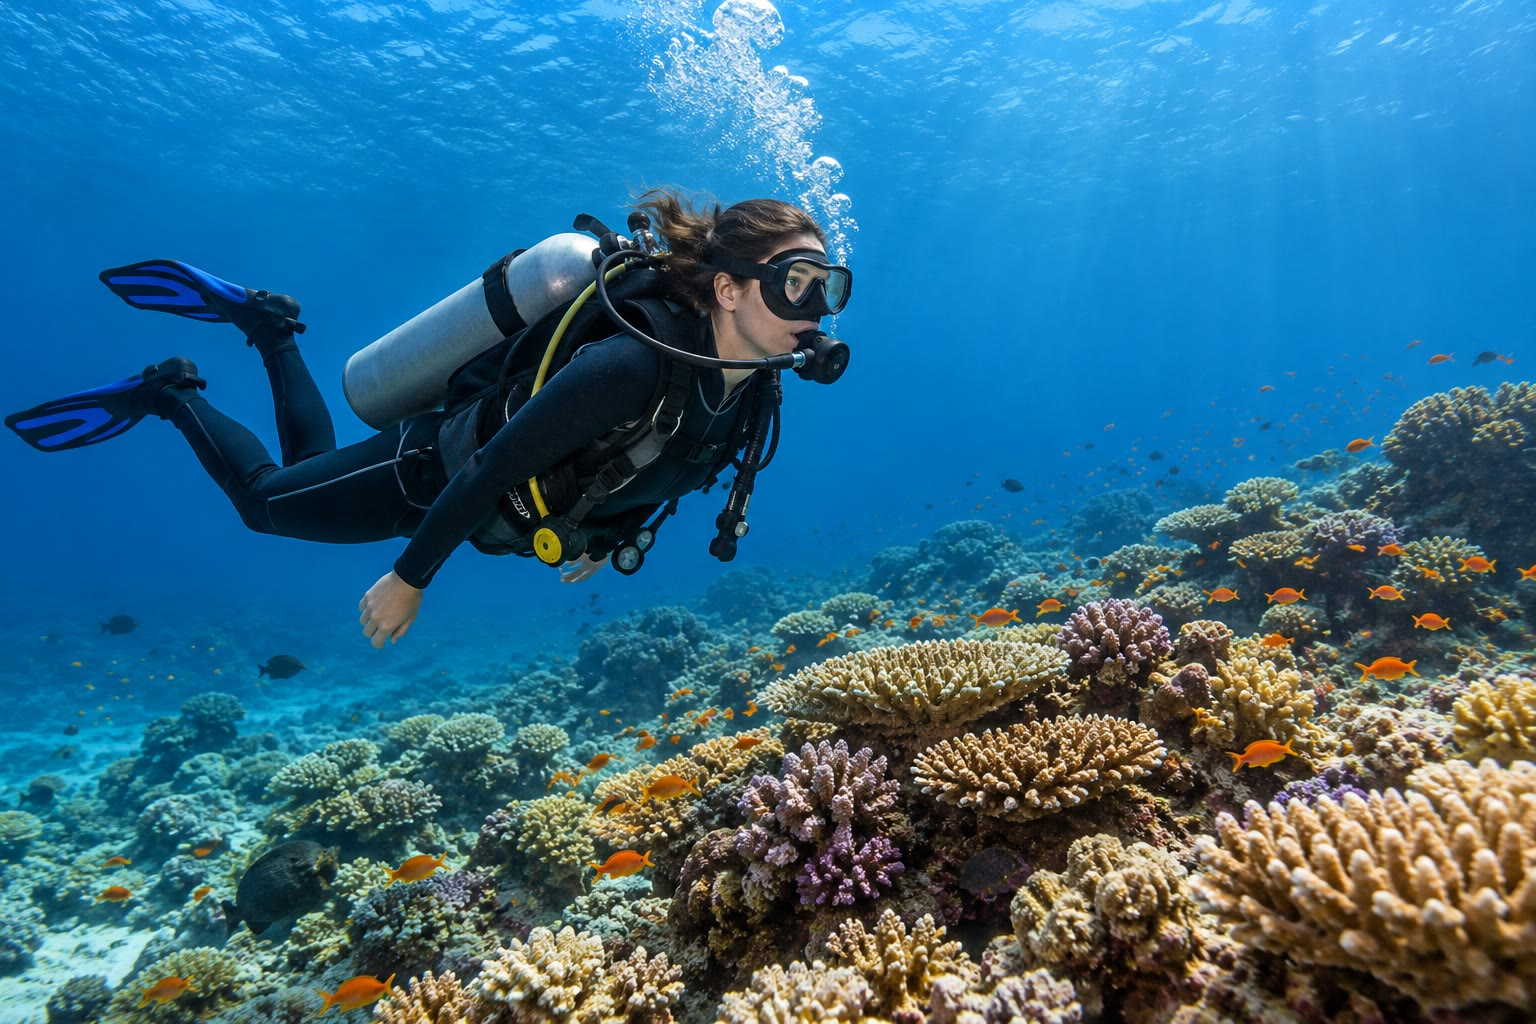
\includegraphics[width=0.55\linewidth]{images/book1/ai/g4-scuba-diver.jpg}

{\small Seorang penyelam menghirup \omterm{def:g4:air-a-mixture-of-gases:air}{udara} dari tabung di punggungnya;
gelembung-gelembung itu adalah \omterm{def:g4:air-a-mixture-of-gases:air}{udara} yang diembuskan.}
\end{omfigure}

\begin{remark}[Mengapa penyelam menghirup udara]\label{rem:g4:air-a-mixture-of-gases:diver}
Tabung penyelam diisi \omterm{def:g4:air-a-mixture-of-gases:air}{udara} yang dimampatkan ke dalam ruang sempit,
bukan oksigen murni: menghirup oksigen murni jauh di bawah air itu
berbahaya. Nitrogen di dalam \omterm{def:g4:air-a-mixture-of-gases:air}{udara} berguna untuk mengencerkan
oksigennya.
\end{remark}

\section{Oksigen untuk kehidupan dan untuk api}

\begin{proposition}[Oksigen dipakai oleh makhluk hidup dan oleh nyala api]\label{prop:g4:air-a-mixture-of-gases:oxygen}
Di antara semua gas di \omterm{def:g4:air-a-mixture-of-gases:air}{udara}, oksigenlah yang diperlukan makhluk hidup
dan nyala api. Hewan dan manusia menghirupnya ketika bernapas; nyala api
mengambilnya dari \omterm{def:g4:air-a-mixture-of-gases:air}{udara} di sekitarnya. Tumbuhan hijau, pada siang hari,
mengembalikan oksigen ke \omterm{def:g4:air-a-mixture-of-gases:air}{udara}.
\end{proposition}

\begin{inthelab}[Lilin di bawah stoples]
Guru menyalakan sebatang lilin di atas sekeping ubin lalu perlahan
menutupinya dengan stoples kaca yang besar. Nyalanya mengecil,
berkedip-kedip, dan padam setelah beberapa detik: di sekitar nyala itu,
\omterm{def:g4:air-a-mixture-of-gases:air}{udara} mengandung terlalu sedikit oksigen untuk membuatnya tetap
menyala. Di bawah stoples yang dua kali lebih besar, lilin menyala
kira-kira dua kali lebih lama, karena ada kira-kira dua kali lebih banyak
\omterm{def:g4:air-a-mixture-of-gases:air}{udara}, jadi dua kali lebih banyak oksigen, untuk dipakai.
\end{inthelab}

\begin{omfigure}
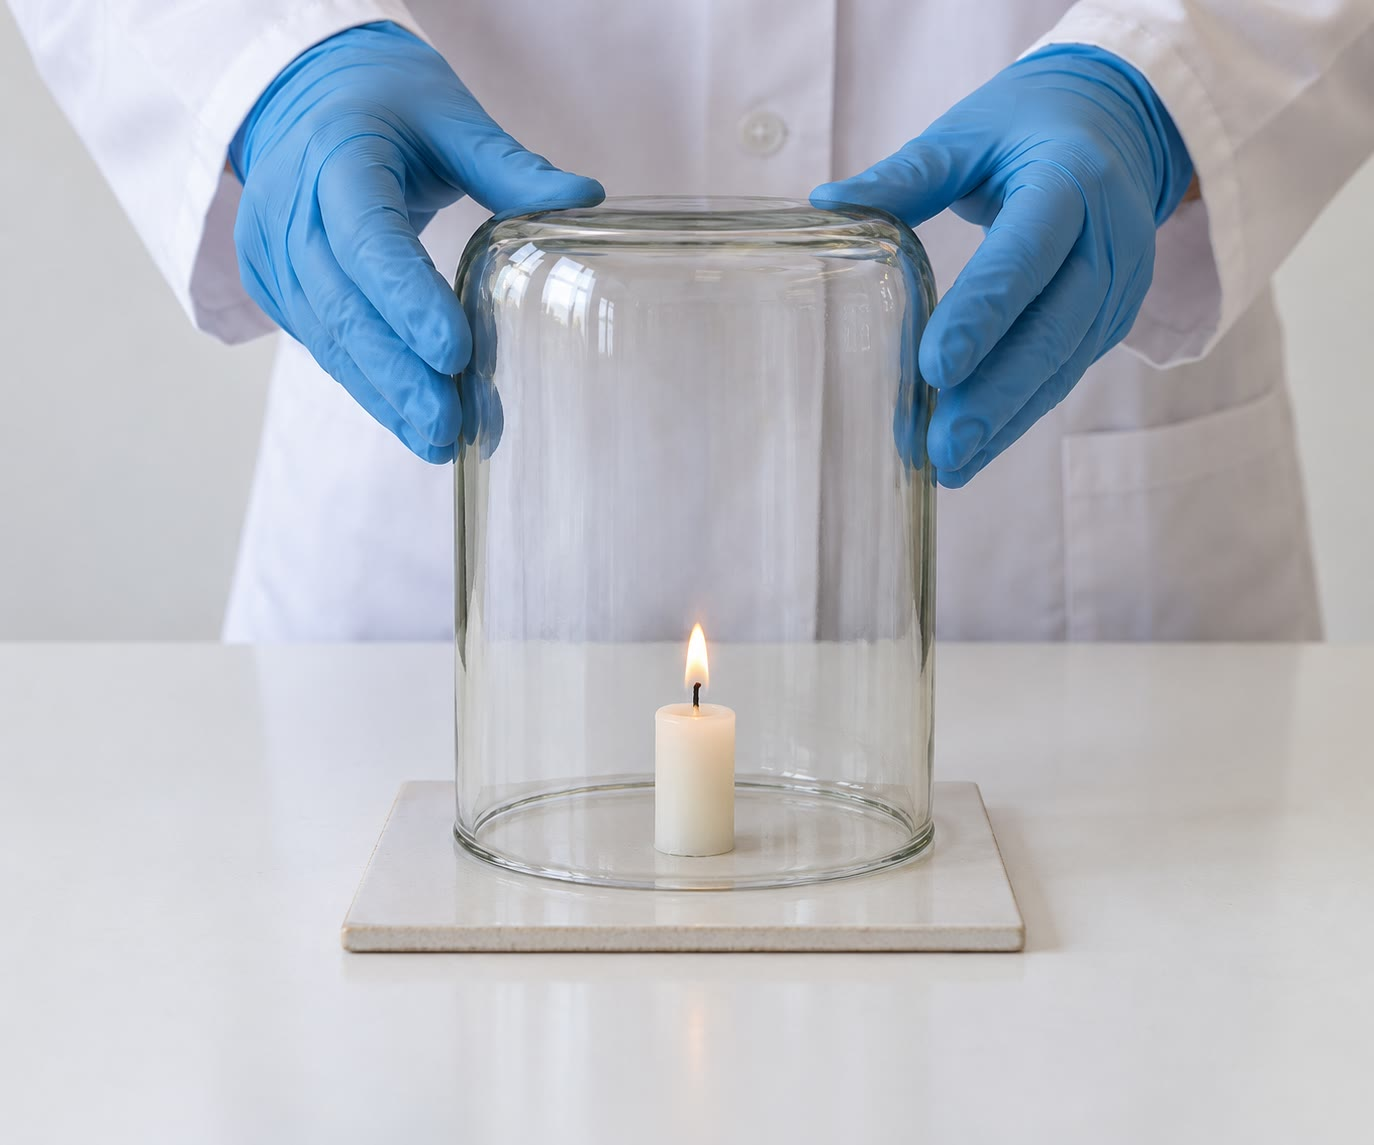
\includegraphics[width=0.5\linewidth]{images/book1/ai/g4-candle-jar-lab.jpg}

{\small Lilin di bawah stoples kaca padam ketika oksigen di sekitar
nyalanya tinggal terlalu sedikit.}
\end{omfigure}

\begin{remark}[Nitrogen tidak terbakar]\label{rem:g4:air-a-mixture-of-gases:nitrogen}
Nitrogen adalah bagian terbesar \omterm{def:g4:air-a-mixture-of-gases:air}{udara}, tetapi nitrogen tidak membuat
nyala api tetap menyala dan tidak dipakai oleh tubuh kita. Seandainya
\omterm{def:g4:air-a-mixture-of-gases:air}{udara} seluruhnya nitrogen, kita tidak dapat bernapas dan tidak ada yang
dapat terbakar.
\end{remark}

\section{Latihan}

\begin{exercise}[$\star$]\label{exo:g4:air-a-mixture-of-gases:1}
Apakah \omterm{def:g4:air-a-mixture-of-gases:air}{udara} satu gas saja atau campuran? Sebutkan dua gas utama di
\omterm{def:g4:air-a-mixture-of-gases:air}{udara}.
\end{exercise}

\begin{exercise}[$\star$]\label{exo:g4:air-a-mixture-of-gases:2}
Kira-kira berapa bagian \omterm{def:g4:air-a-mixture-of-gases:air}{udara} yang berupa nitrogen? Kira-kira berapa
bagian yang berupa oksigen?
\end{exercise}

\begin{exercise}[$\star$]\label{exo:g4:air-a-mixture-of-gases:3}
Dalam 100 liter \omterm{def:g4:air-a-mixture-of-gases:air}{udara} kering, kira-kira berapa liter yang berupa
nitrogen? Kira-kira berapa liter yang berupa oksigen?
\end{exercise}

\begin{exercise}[$\star$]\label{exo:g4:air-a-mixture-of-gases:4}
Sebuah botol kosong dimasukkan terbalik ke dalam baskom berisi air.
Mengapa air tidak memenuhi botol itu?
\end{exercise}

\begin{exercise}[$\star$]\label{exo:g4:air-a-mixture-of-gases:5}
Lihatlah diagram batang. Gas apa yang lebih sedikit dalam \omterm{def:g4:air-a-mixture-of-gases:air}{udara} yang
diembuskan? Gas apa yang lebih banyak?
\end{exercise}

\begin{exercise}[$\star$]\label{exo:g4:air-a-mixture-of-gases:6}
Gas apa di \omterm{def:g4:air-a-mixture-of-gases:air}{udara} yang diperlukan nyala api? Gas apa di \omterm{def:g4:air-a-mixture-of-gases:air}{udara} yang kita
perlukan ketika bernapas?
\end{exercise}

\begin{exercise}[$\star$]\label{exo:g4:air-a-mixture-of-gases:7}
Lihatlah gambar dengan 100 kotak. Berapa kotak yang berupa nitrogen?
Berapa kotak yang bukan nitrogen?
\end{exercise}

\begin{exercise}[$\star$]\label{exo:g4:air-a-mixture-of-gases:8}
Mengapa lilin di bawah stoples padam setelah beberapa saat?
\end{exercise}

\begin{exercise}[$\star$]\label{exo:g4:air-a-mixture-of-gases:9}
Dalam 500 liter \omterm{def:g4:air-a-mixture-of-gases:air}{udara}, kira-kira berapa liter yang berupa oksigen?
(Seperlima \omterm{def:g4:air-a-mixture-of-gases:air}{udara} adalah oksigen.)
\end{exercise}

\begin{exercise}[$\star\star$]\label{exo:g4:air-a-mixture-of-gases:10}
Mengapa membuka jendela ruang kelas di antara jam pelajaran itu baik?
\end{exercise}

\begin{exercise}[$\star\star$]\label{exo:g4:air-a-mixture-of-gases:11}
Sebatang lilin menyala selama 10 detik di bawah stoples kecil.
Kira-kira berapa lama lilin itu akan menyala di bawah stoples yang berisi
\omterm{def:g4:air-a-mixture-of-gases:air}{udara} tiga kali lebih banyak?
\end{exercise}
